\section{ContinuumBDT}
\label{sec:ContinuumBDT}
% \newcommand{\Bsmumu}{\ensuremath{B_s^0 \to \mu^+\mu^-}\xspace}

In order to discriminate against the continuum background we
employ a Multi-Variate Analysis (MVA) strategy, based on a boosted decision tree (BDT)
algorithm, as implemented in the TMVA~\cite{Hoecker:TMVA} package of ROOT. We use
$15$ physical input variables to obtain the signal-to-background discriminator. These  $15$ input 
variables are summarised in Table~\ref{tab:15vars} along with a short description of each variable.
The BDT ranking of input variable importance is given in Table ~\ref{tab:VarImportance} and compared to 
the separation power of the signal and background.
  
The following summarises the input variables which were considered for use in the
BDT. After discussing the individual variables, details of training and validation
of the classifier are given.
  
The variables can be subdivided into two groups, one related to isolation properties
of the $B$ candidates or the final state particles, and another describing topological
and kinematic properties of the \Bsmumu decay.
  
To check the isolation of the signal decay we look at non-signal tracks in the vicinity
of reconstructed B vertices, excluding the tracks associated to the pile-up vertices.
The procedure of computation of the variable, outlined in section~\ref{ssec:CandidateBuildingByDerivation} 
requires information from all tracks in an event and therefore performed on the derivation level.

\yel[t.b.c.]{Since individual muons in the signal decay are fairly well separated, isolation variables
of individual muon candidates have also been considered. However, they were rejected
in the final training, since the $B$ isolation variable $I_{0.7}$, highly correlated
to the single-muon isolation variables, contains nearly all the separation power of this
type of variables by itself.}
  
% In the computation of the $I_{0.7}$ variable we employ our own track-to-PV association
% algorithm, similar to the $B$ vertex association described above. In this way, the
% $I_{0.7}$ variable results to be robust against pile-up events. The corresponding
% requirement on the track-to-PV association was re-optimised due to the larger pile-up
% in 2012 data. We have tightened the cut on the $\ln\chi^2$ value to be less than $5$
% (instead of $6$ used in the analysis of 2011 data), which gave the best performance
% in signal/background separation.
  
The other $12$ variables in Table~\ref{tab:15vars} are related to B-decay topology and
kinematics. They were chosen from the larger pool of variables as the ones ensuring
the best BDT performance.
The variables that have been considered but dismissed are listed below for future
reference: they do not contribute significantly to the signal/background separation,
either by nature or due to the presence of other strongly correlated but more powerful
variables.
   
\begin{itemize}
\setlength{\itemsep}{0pt}%
\setlength{\parskip}{0pt}%
\item $L_{xy}$ significance
\item flight length significance in 2D and 3D
\item $d_0^{Max}$, $d_0^{Min}$
\item the significance of the closest track DOCA
\item $\chi^2$ between PV and B vertex in $z$ 
\item $p_{T}^{B}$ significance
%$B$ transverse momentum significance
% 1 BvtxPointingAngle3D a_3D pointing angle in 3D 
\item   pointing angle $|\alpha_{3D}|$
%       Absolute value of the angle between $\Delta\overrightarrow{x}$ and $\overrightarrow{p}^{B}$ & new \\ \\
% 15 BvtxChi2byNDF B_fitChi2NDF chi2/NDF of B vertex 
\item B vertex fit $\chi^2_B$/NDF
%$\chi^2$/NDF of the $B$ vertex & new \\
\item coplanarity of \Bsmumu' decays
\item coplanarity of \Bsmumu' decays with $Z$-axis
\item minimum signed $d_0$ significance of the signal candidate
\end{itemize}
Lastly in order to arrive at the BDT to
use for this analysis, a number of configurations have been studied, and
the best (with respect to background rejection and algorithm behavior)
has been selected for use in the final result.
 
\begin{table}[!htb]
\begin{center}
\begin{tabular}{p{2cm} p{10.9cm} p{2.1cm}}
\hline \hline
Variable  &  Description \\ 
\midrule
% 1. TMath::Abs(BvtxPointingAngle2D) TMath::Abs(a_2D) angle btw. dX and pB in xy plane used in 2011 analysis
$|\alpha_{2D}|$ & Absolute value of the angle in the transverse plane
between $\Delta\overrightarrow{x}$ and $\overrightarrow{p}^{B}$ \\ \\   
% 2. BvtxIsolation B_iso_7_Chi2_5_MedPt05 isolation of B candidate used in 2011 analysis(*)
Isolation $I_{0.7}$ & Ratio of $|\overrightarrow{p}^{B}_{T}|$ to the sum of $|\overrightarrow{p}^{B}_{T}|$ and
the transverse momenta of all tracks with $p_T > 0.5$ GeV within a
cone $\Delta{R} < 0.7$ from the $B$ direction, excluding $B$ decay products  \\ \\  
% 3. BvtxDR DR sqrt(df^2+deta^2) btw. dX and pB used in 2011 analysis
$\Delta{R}$ & Angle $\sqrt{\left(\Delta\phi\right)^{2} + \left(\Delta\eta\right)^{2}} $
between $\Delta\overrightarrow{x}$ and $\overrightarrow{p}^{B}$ \\ \\  
% 4.  BvtxPt B_pT pT of B candidate used in 2011 analysis
$p_{T}^{B}$ & $B$ transverse momentum  \\ \\  
% 5.  minChi2MuonsIP2AnyPV B_minChi2MuonsIPtoAnyPV
$\chi^2_{\mu,xPV}$ & Minimum $\chi^2$ between the muon candidates and any PV  \\  
% 6. lnChi2PVtxBVtx2D chi2_PVSV_log2D chi2 btw. PV and SV in xy used in 2011 analysis
%        $\chi^{2}_{z}, \chi^{2}_{xy}$ & Significance of the separation between production
%        (PV) and decay (SV) vertices, $\Delta\overrightarrow{x}^{T}\cdot
%        \left(\sigma^{2}_{\Delta\overrightarrow{x}}\right)^{-1}\cdot\Delta\overrightarrow{x}$,
%        in $z$ and $(x,y)$, respectively & used in $2011$\\ \\
$\log[\chi^{2}_{\mathrm{PV,SV}}]_{xy}$ & separation between production
(PV) and decay (SV) vertices, $\Delta\overrightarrow{x}^{T}\cdot
\left(\sigma^{2}_{\Delta\overrightarrow{x}}\right)^{-1}\cdot\Delta\overrightarrow{x}$,
in the transverse plane $(x,y)$ \\ \\  
% 7. Bvtx3DIP Bvtx3DIP 3D impact parameter (POCA) of B candidate
IP$_B^{3D}$ & 3-dimensional impact parameter (POCA) of the $B$ candidate \\  
% 8. TMath::Abs(d0MaxSign) d0Max_sig IP significance of the muon track with max IP
$|d_{0}|^{max}$ sig. & Significance of the maximum absolute value of impact
parameters of the two muon candidates in the transverse plane of the $B$
decay products relative to the primary vertex \\  
% 9. TMath::Abs(MuonsRefTrksDPhi) B_IDtrks_deltaPhi &Delta(&phi,&mu1 - &phi,&mu2)
$\Delta\phi(\mu\mu)$ & Difference in $\phi$ between the two muon candidates  \\  
% 10. ClosTrackDOCA closeTrkDOCA DOCA of the track closest to B vertex
DOCA$_{xtrk}$ & DOCA of the track closest (``xtrk'') to the $B$ vertex.
The tracks associated to pile-up vertices are excluded \\  
% 11. TMath::Abs(MuonsDCA) TMath::Abs(B_IDtrks_DCA) DCA ot two ID tracks forming B vertex
DOCA$_{\mu\mu}$ & DOCA of the two ID tracks forming the $B$ vertex  \\  
% 12. ClosTrackNTracksChi2 closeTrkNtrksChi2 chi2 btw. the closest track and B vertex
%        $\chi^2_{B,xtrk}$ & $\chi^2$ between the closest track and the $B$ vertex  & new \\
$N^{close}_{trks}$ & Number of (``close'') tracks with $\ln(\chi^2)<1$ where
$\chi^2$ is a test of association of a track to the reconstructed $B$ vertex.
The tracks associated to pile-up vertices are excluded\\  
% 13. TMath::Abs(d0MinSign) d0Min_sig IP significance of the muon track with min IP
$|d_{0}|^{min}$ sig. & Significance of the minimum absolute value of impact
parameters of the two muon candidates in the transverse plane of the $B$
decay products relative to the primary vertex\\  
% 14. BvtxLxy Lxy (dxp)xy/pt used in 2011 analysis
$L_{xy}$ & Scalar product in the transverse plane of
$(\Delta\overrightarrow{x}\cdot\overrightarrow{p}^{B})/|\overrightarrow{p}^{B}_{T}|$\\ \\  
% 15. BvtxPlngMin2D PlngMin2D minimum momentum of the two muon candidates along the B direction used in 2011 analysis
%        $P_{L}^{min}, P_{L}^{max}$ & Minimum and maximum momenta of
%        the two muon candidates along the $B$ direction & used in $2011$\\ \\
$P_{L}^{min}$ & Minimum momentum of the two muon candidates
along the $B$ direction\\ \\
\hline \hline
\end{tabular}
\caption{Description of the $15$ discriminating variables used in the
discrimination between signal and continuum background.}
\label{tab:15vars}
\end{center}
\end{table}

\begin{table}[!htb]
\begin{center}
%CMD+l lift then press j - sync to pdf on skim
%on skim CMD-Shift click - sync back to ST (sublime text)
%build latex with CMD+b
%CMD+l lift then press delete - remove aux files from folder!!
%Installed LaTexTools and LaTex-clw for autocomplete

\documentclass[12pt]{article} %[12pt]
%compile using LuaLaTex from drop down menu
% comment multiple lines using \iffalse *multiple lines of text*  \fi
\usepackage{tikz}
\usepackage{tikz-feynman}
\tikzfeynmanset{compat=1.0.0}
\usepackage{caption}
\usepackage{subcaption}
\usepackage{float}
%\usepackage{atlasphysics}
%Bibliography preamble
\usepackage[numbers,sort&compress]{natbib}
%geometry of margins
\usepackage[left=1in,right=1in,top=1in,bottom=0.5in]{geometry}
\usepackage{url}
\usepackage{amsmath}
\usepackage{bm}
\usepackage{amssymb}
\usepackage{mathtools}
\usepackage[utf8]{inputenc}
\usepackage{longtable}

\newcommand*{\TitleFont}{%
      %\usefont{\encodingdefault}{\rmdefault}{b}{n}%
      \fontsize{16}{20}%
      \selectfont}
%\date{December 15, 2016}
\usepackage{booktabs}
\usepackage{longtable}
\usepackage{array}
\usepackage{lscape}
\begin{document}
\begin{landscape}
\begin{longtable}{llrlr}
\toprule
Imp. Rank &                                       Variable &  Importance & Sep. Rank &  Separation \\
\midrule
\endhead
\midrule
\multicolumn{3}{r}{{Continued on next page}} \\
\midrule
\endfoot

\bottomrule
\endlastfoot
        1 &                                $|\alpha_{2D}|$ &     0.11290 &         2 &     0.57270 \\
        2 &                                     $\Delta R$ &     0.10720 &         1 &     0.59070 \\
        3 &         B Iso BEJ (PPP) Custom TVA Trk Perigee &     0.09343 &         6 &     0.39280 \\
        4 &                      $log(\chi^{2}_{\mu,xPV})$ &     0.08988 &         4 &     0.43970 \\
        5 &                            $ln(\chi^{2}_{xy})$ &     0.07679 &         9 &     0.30400 \\
        6 &                                      $p^B_{T}$ &     0.07132 &        13 &     0.02416 \\
        7 &                       $|\Delta \phi_{\mu\mu}|$ &     0.06958 &        15 &     0.01313 \\
        8 &  nCloseTracks BEL (PPP) Custom TVA Trk Perigee &     0.06658 &         3 &     0.45130 \\
        9 &                                $|IP_{B}^{3D}|$ &     0.05015 &        11 &     0.14500 \\
       10 &                                $DOCA_{\mu\mu}$ &     0.04812 &        12 &     0.07437 \\
       11 &          DOCA BEL (PPP) Custom TVA Trk Perigee &     0.04766 &         5 &     0.40100 \\
       12 &                                       $L_{xy}$ &     0.04485 &         8 &     0.37820 \\
       13 &                                  $P^{min}_{L}$ &     0.04410 &        14 &     0.02359 \\
       14 &                               $d^0_{max, sig}$ &     0.04252 &        10 &     0.17100 \\
       15 &                               $d^0_{min, sig}$ &     0.03502 &         7 &     0.39140 \\
\end{longtable}

\end{landscape}
\end{document}
\caption{The BDT ranking of input variable importance and compared with the signal and background 
separation power of each variable as calculated by TMVA before training.}
\label{tab:VarImportance}
\end{center}
\end{table}
 
Appendix~\ref{app:contBDT} summarises the correlation matrices calculated
for signal and background events for the $15$ discriminating variables used
in this analysis.
The BDT training is done using the \bbmumuX background MC (described in
%used to be sec:4corners
Sec.~\ref{sec:BackgroundModeling}) and signal MC events. All selection cuts are applied to both the combinatorial events and the signal MC events. 
 
The training is done using the TMVA tool, splitting the two input samples into
equal halves. The first half is used for training the BDT and the second for
validation.
The $1/4$th of the signal MC was kept off the training and validation samples and
it has been used for evaluation, together with the data candidates from the right
mass sideband.\footnote{To clarify, the signal MC sample events are used:
$37.5\%$ for training, $37.5\%$ for validation, and $25\%$ for evaluation.}
The left plot in Figure~\ref{fig:contBDT} shows the test for over-training,
where the BDT outputs for training and validation samples are shown, confirming that
the BDT is not over-trained as the training and validation samples are in good
agreement with each other. \yel[t.b.d.]{The right plot contains the training result via
the Receiver Operating Characteristic (ROC) curve and the comparison with the BDT
used in 2012 analysis: the new training results to be significantly more efficient.}
 
\begin{table}[htbp]
\begin{center}
\begin{tabular}{|c|c|}
\hline
Parameter & Value \\
\hline
\hline
\textit{NTrees} & 500 \\
\hline
\textit{MinNodeSize} & 1.0[\%]\\
\hline
\textit{MaxDepth} & 3 \\
\hline
\textit{BoostType} & AdaBoost \\
\hline
\textit{AdaBoostBeta} & 0.5 \\
\hline
\textit{UseBaggedBoost} & True\\
\hline
\textit{BaggedSampleFraction} & 0.6\\
\hline
\textit{SeparationType} & GiniIndex \\
\hline
\textit{nCuts} & 100\\
\hline
\textit{NormMode} & EqualNumEvents\\
\hline
\hline
\end{tabular}
\end{center}
\caption{\label{tab:cBDTPars} Configuration parameters of the \textit{continuum}-BDT.}
\end{table}
 
The final choice of the configuration parameters of the \textit{continuum}-BDT,
as used by TMVA, is shown in Table \ref{tab:cBDTPars}.
The optimal values for the configuration parameters \textit{MinNodeSize} 
and \textit{AdaBoostBeta} were found with the help of a grid scan using background rejection at 36\% signal efficiency on the ROC-curve as a figure of merit of classifier performance. The \textit{MaxDepth} parameter
has also been studied in the similar way. For this parameter, it has been found
that the performance of classifier improves with increasing
of \textit{MaxDepth}, whereas the discrepancy between its performance on the training
and testing sample, accessed by the Kolmogorov-Smirnov test, becomes larger,
leading to the over-training. In order to not compromise the generality of the classifier,
the value \textit{MaxDepth=3} has been chosen.
The value of \textit{NTrees} has been chosen large enough to allow the training to converge.
The choice of other parameters does not have any significant impact on the training result.
 
We have tested the chosen BDT configuration against different training samples including
various sample re-weighting, previous selection cuts and increase of statistics.
We found no real impact on the performance of the BDT proving that the chosen
configuration is very robust.
 
\yel[t.b.c.]{In addition we tested a BDT variable built without the use of the isolation variable
as input: the study is described in Appendix}~\ref{app:BDT-noISO}. As expected, the
separation power is reduced thus the BDT configuration described in this section is
the one used in the analysis.
 
\begin{figure}[!htb]
\begin{center}
\hspace{-0.5cm}
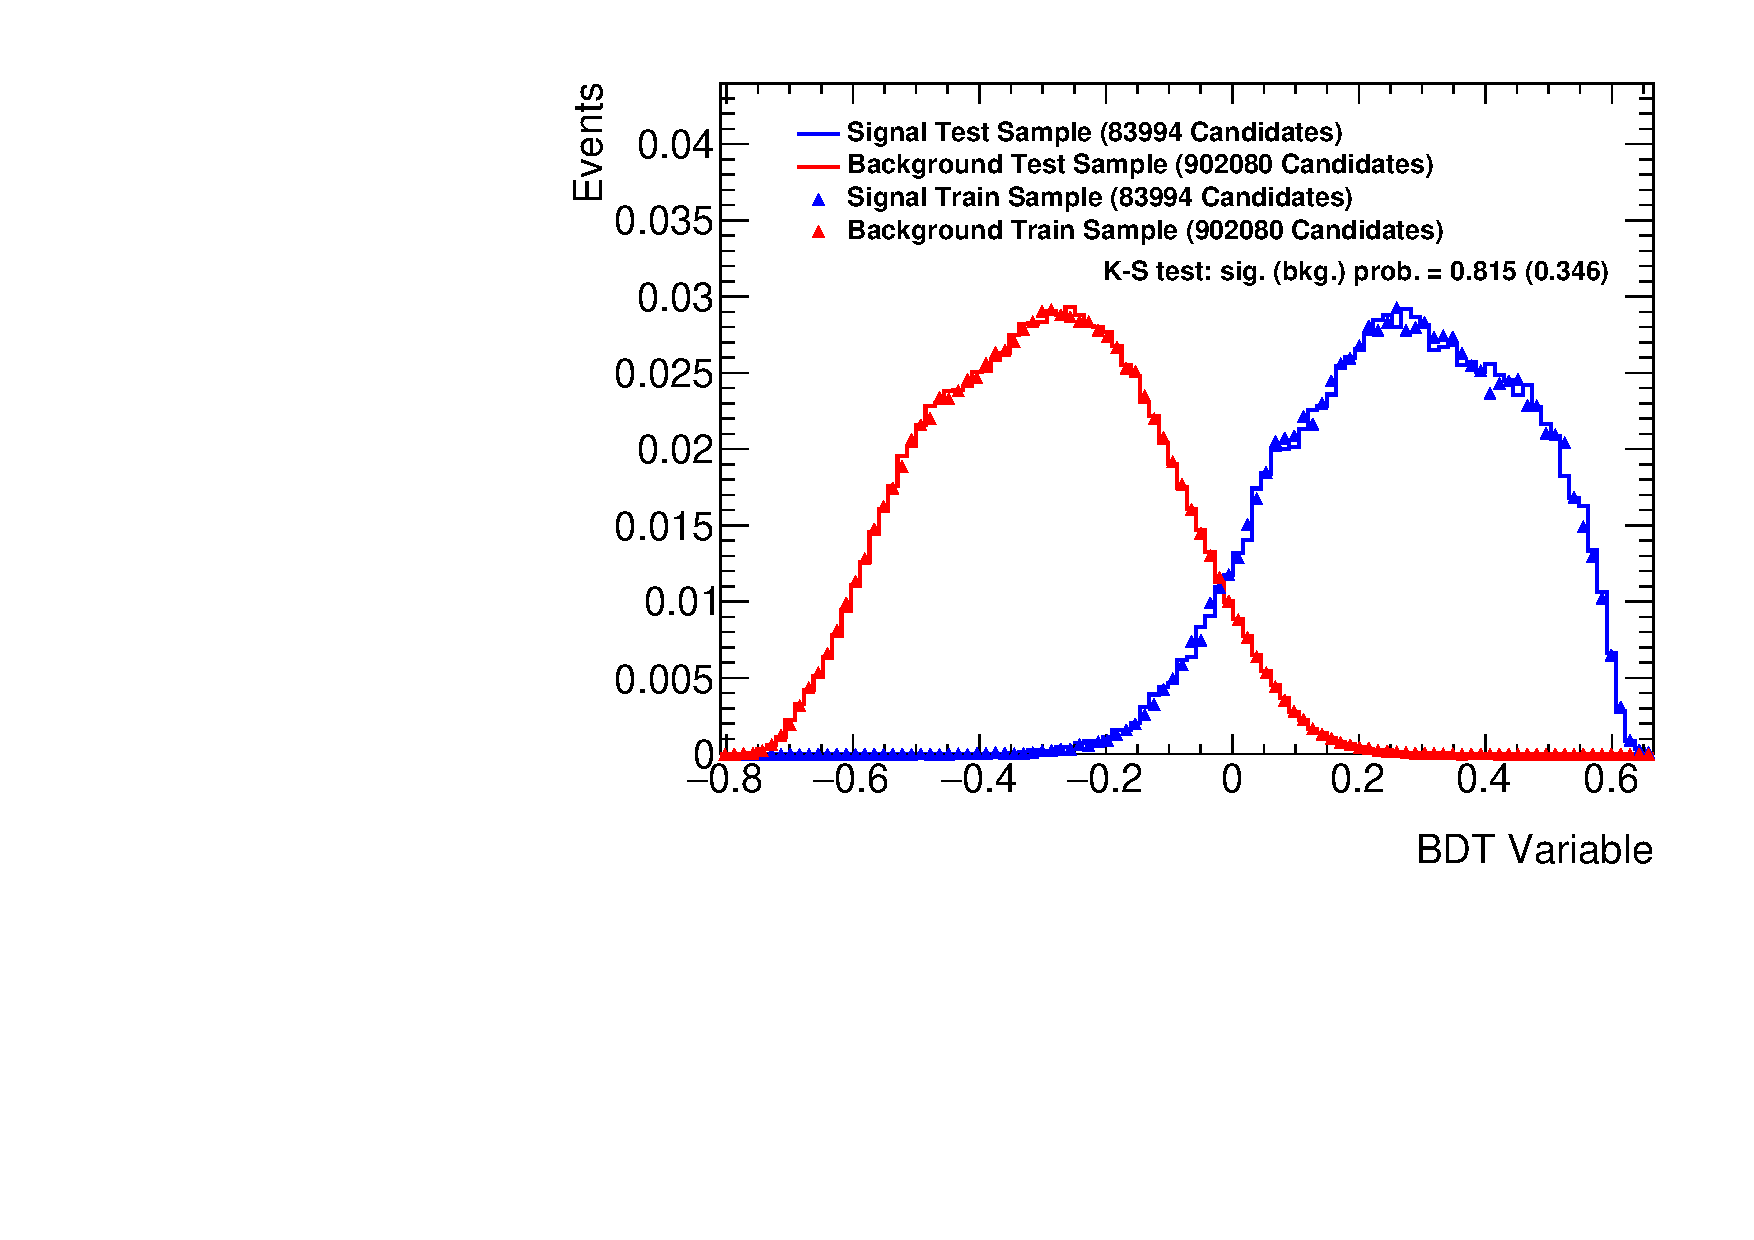
\includegraphics[width=0.52\textwidth]{figures/InternalNote_ContinuumBDT/KS.pdf}
\hspace{-0.5cm}
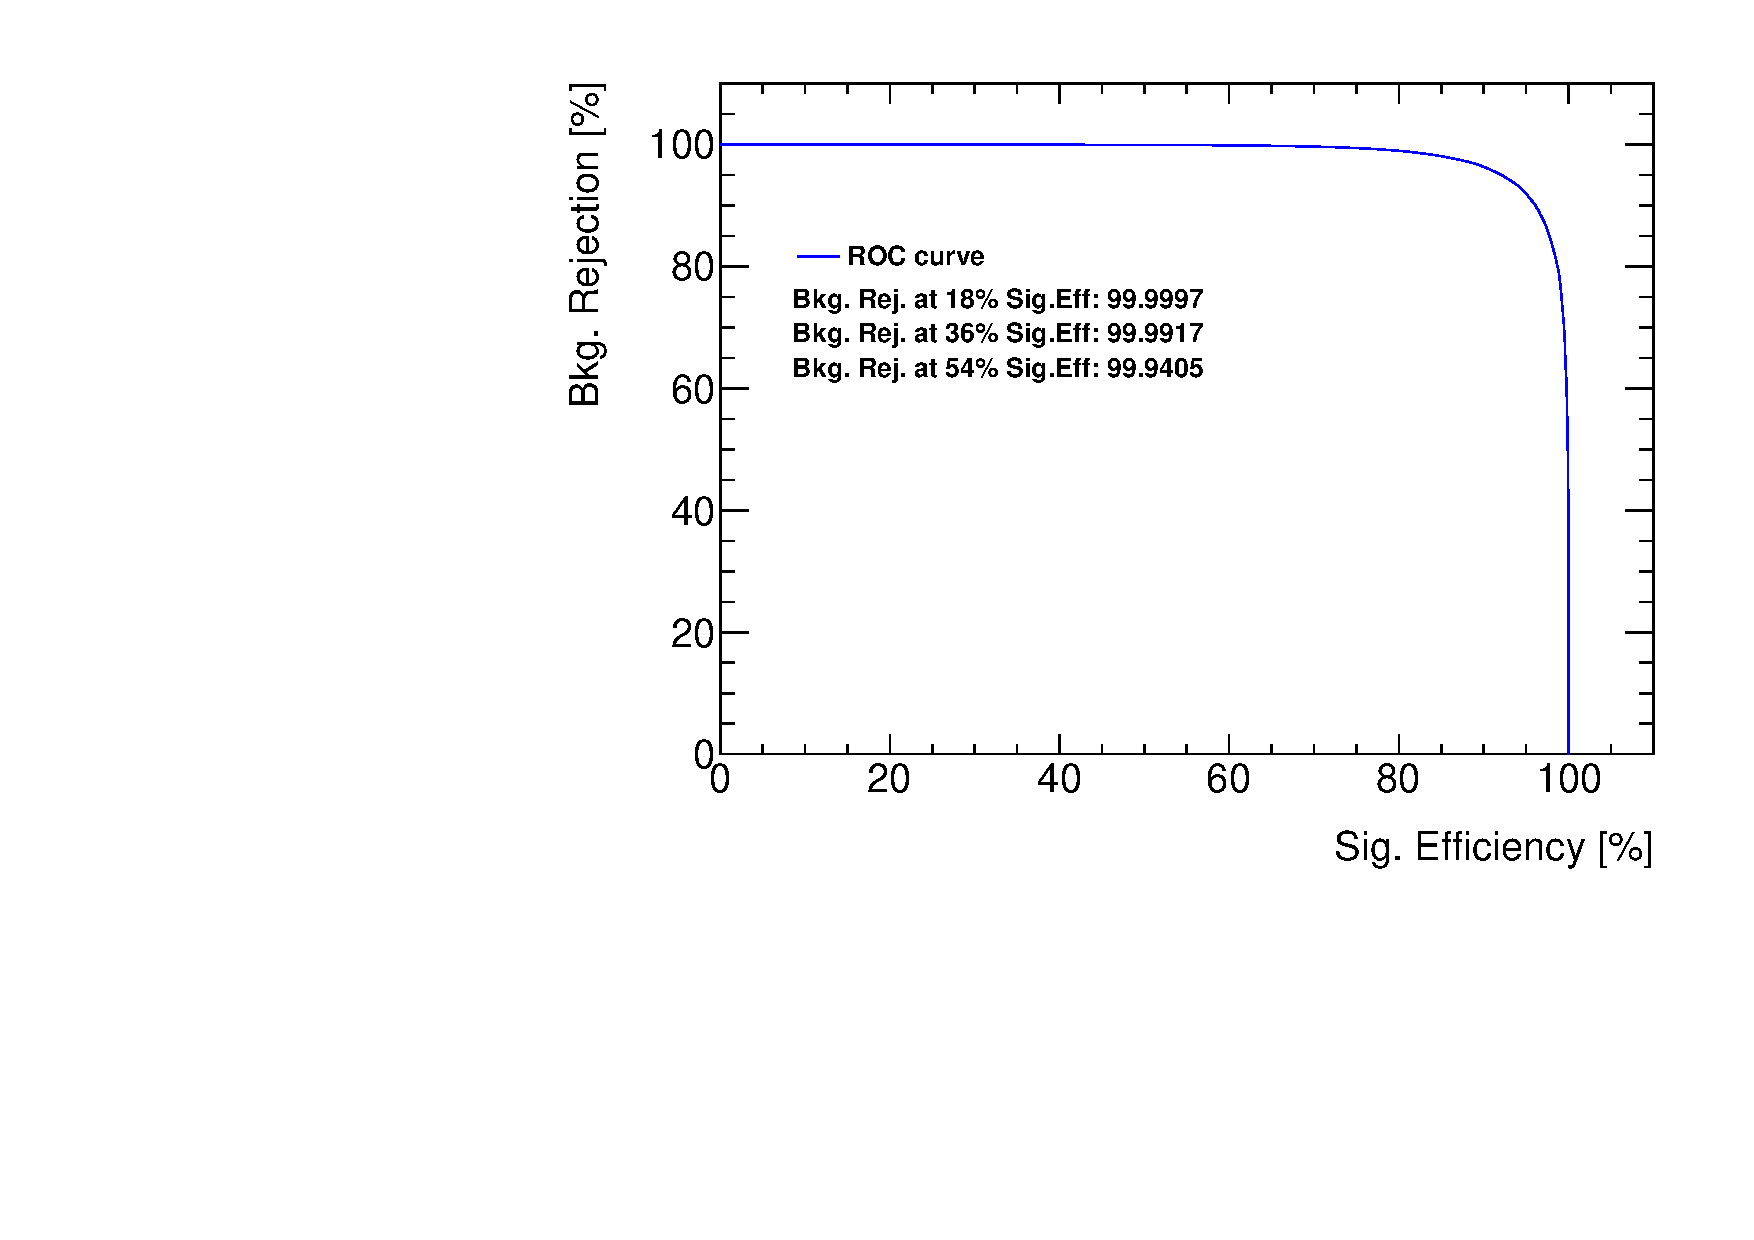
\includegraphics[width=0.52\textwidth]{figures/InternalNote_ContinuumBDT/ROC.pdf}
\caption{{\itshape Left}: cross-checks for over-training for the continuum BDT variable.
{\itshape{Right}}: \textbf{Only ROC curve at the moment!} comparison of ROC curves trained on the combinatorial background MC and the signal MC. The ROCs are evaluated on the high-mass data sideband.}
\label{fig:contBDT}
\end{center}
\end{figure}



\clearpage
